\documentclass{article}
\usepackage{amsmath}
\usepackage{graphicx}
\usepackage{float}
\usepackage[utf8]{inputenc}
\usepackage{listings}
\usepackage{color}
\definecolor{deepblue}{rgb}{0,0,0.5}
\definecolor{deepred}{rgb}{0.6,0,0}
\definecolor{deepgreen}{rgb}{0,0.5,0}
\usepackage{graphicx}
\usepackage{caption}
\usepackage{subcaption}

\usepackage[a4paper]{geometry}
\geometry{
left = 20mm,
right = 20mm,
top = 20mm,
bottom = 20mm,
}

\usepackage[backend=bibtex,
style=numeric,
bibencoding=ascii
%style=alphabetic
%style=reading
]{biblatex}
\addbibresource{biblio.bib}


\usepackage[]{listings
}
% Python style for highlighting
\newcommand\pythonstyle{\lstset{
language=Python,
basicstyle=\ttm,
otherkeywords={self},             % Add keywords here
keywordstyle=\ttb\color{deepblue},
emph={MyClass,__init__},          % Custom highlighting
emphstyle=\ttb\color{deepred},    % Custom highlighting style
stringstyle=\color{deepgreen},
frame=tb,                         % Any extra options here
commentstyle=\color{deepred},%
showstringspaces=false            % 
}}

\usepackage{hyperref}
\usepackage{color}



\begin{document}
%%%%%%%%%%%%%%%%%%%%%%%%%%%%%%%%%%%%%%%%%
% University Assignment Title Page 
% LaTeX Template
% Version 1.0 (27/12/12)
%
% This template has been downloaded from:
% http://www.LaTeXTemplates.com
%
% Original author:
% WikiBooks (http://en.wikibooks.org/wiki/LaTeX/Title_Creation)
%
% License:
% CC BY-NC-SA 3.0 (http://creativecommons.org/licenses/by-nc-sa/3.0/)
% 
% Instructions for using this template:
% This title page is capable of being compiled as is. This is not useful for 
% including it in another document. To do this, you have two options: 
%
% 1) Copy/paste everything between \begin{document} and \end{document} 
% starting at \begin{titlepage} and paste this into another LaTeX file where you 
% want your title page.
% OR
% 2) Remove everything outside the \begin{titlepage} and \end{titlepage} and 
% move this file to the same directory as the LaTeX file you wish to add it to. 
% Then add \input{./title_page_1.tex} to your LaTeX file where you want your
% title page.
%
%%%%%%%%%%%%%%%%%%%%%%%%%%%%%%%%%%%%%%%%%

%----------------------------------------------------------------------------------------
%	PACKAGES AND OTHER DOCUMENT CONFIGURATIONS
%----------------------------------------------------------------------------------------

\begin{titlepage}

\newcommand{\HRule}{\rule{\linewidth}{0.5mm}} % Defines a new command for the horizontal lines, change thickness here

\center % Center everything on the page
 
%----------------------------------------------------------------------------------------
%	HEADING SECTIONS
%----------------------------------------------------------------------------------------

\textsc{\LARGE Technical University of Denmark}\\[1.5cm] % Name of your university/college
\textsc{\Large Constrained Optimization}\\[0.5cm] % Major heading such as course name
\textsc{\large Course 02612}\\[0.5cm] % Minor heading such as course title

%----------------------------------------------------------------------------------------
%	TITLE SECTION
%----------------------------------------------------------------------------------------

\HRule \\[0.4cm]
{ \huge \bfseries Assignment 1}\\[0.4cm] % Title of your document
\HRule \\[1.5cm]
 
%----------------------------------------------------------------------------------------
%	AUTHOR SECTION
%----------------------------------------------------------------------------------------
\Large \emph{Authors:}\\
Jakub \textsc{Czerny}, s99999\\[10pt]
Oskar \textsc{Hint}, s161559\\[10pt]
Joachim Finn \textsc{Jensen}, s134052\\[10pt]


%\Large \emph{Collaborator:}\\
%some \textsc{collaborator}, s161559\\[2cm] % Your name

%----------------------------------------------------------------------------------------
%	DATE SECTION
%----------------------------------------------------------------------------------------

{\large \today }\\[2cm] % Date, change the \today to a set date if you want to be precise

%----------------------------------------------------------------------------------------
%	LOGO SECTION
%----------------------------------------------------------------------------------------
\vspace{4cm}
\begin{center}
%\includegraphics[width=0.5\textwidth]{fig/dtufotoniklogo.png}
\includegraphics{fig/DTU_3_CMYK.eps}
\end{center}
 % Include a department/university logo - this will require the graphicx package
 
%----------------------------------------------------------------------------------------

\vfill % Fill the rest of the page with whitespace

\end{titlepage}

\newpage
\tableofcontents
\thispagestyle{empty}
\setcounter{page}{0}
\newpage

\section{Assignment}

\subsection{Problem 1 - Quadratic Optimization}
From the problem 1 it is seen that the system can be written as:
\[H=\begin{bmatrix}
	6 & 2 & 1 \\2 & 5 & 2 \\1 & 2 & 4
\end{bmatrix}\]
\[g=\begin{bmatrix}
	-8 \\-3 \\ -3
\end{bmatrix}\]
\[A=\begin{bmatrix}
	1 & 0 \\ 0 & 1 \\ 1 & 1
\end{bmatrix}\]
\[b= \begin{bmatrix}
	3 \\ 0
\end{bmatrix}\]
Then the general KKT system can be written as:
\[\begin{bmatrix}
	H & -A \\A^T & 0
\end{bmatrix} \times \begin{bmatrix}
	x\\ \lambda
\end{bmatrix} =\begin{bmatrix}
	-g\\ b
\end{bmatrix}\]
Which in this case can be written as:
\[\begin{bmatrix}
	6 & 2 & 1 & -1 & 0\\2 & 5 & 2 & 0 & -1\\1 & 2 & 4 & -1 & -1 \\
1 & 0 & 1 & 0 & 0\\ 0 & 1 & 1 & 0 & 0
\end{bmatrix} \times \begin{bmatrix}
	x_1 \\ x_2 \\ x_3 \\ \lambda_1 \\ \lambda_2
\end{bmatrix} =\begin{bmatrix}
	8 \\3 \\ 3\\ 3 \\ 0
\end{bmatrix}\]
The system is solved in MatLab by making a function that solves the problem by use of the backslash command, see the code how it was done. The result shows that:
\[x=\begin{bmatrix}
	2 \\ -1 \\ 1
\end{bmatrix}\]
\[\lambda=\begin{bmatrix}
	3 \\ 2 
\end{bmatrix}\]
To test the solver, random values for x and $\lambda$ are generated, from these the H, g, A and b are determined. With these matrix and vectors the system are solved again. If the function finds the same x and lambda that were previously randomly chosen, the solver works. Our solver works as expected and gives the same values for x and lambda that were generated.\\
To see the sensitivity of the problem parameter sensitivity analysis is conducted. The general function is as followed. 
\[F(x,\lambda;p)= \begin{bmatrix}
	\nabla_x f(x,p)- \nabla_x c(x,p)\lambda \\ c(x,p)
\end{bmatrix}=\begin{bmatrix}
0 \\ 0
\end{bmatrix}\]
Where the implicit function theorem gives parameter sensitivities
\[[\nabla_x(p) \lambda(p)]=-[W_{xp} -\nabla_p c(x,p)\begin{bmatrix}
W_{xx} & -\nabla_x c(x,p) \\ -\nabla_x c(x,p)^T & 0
\end{bmatrix}^{-1}\]
\[ W_{xx} = \nabla^2_{xx} f(x,p) - \sum\limits_{i\in\varepsilon} \lambda_i\nabla^2_{xx}c_i(x,p)\]
\[ W_{xp} = \nabla^2_{xp} f(x,p) - \sum\limits_{i\in\varepsilon} \lambda_i\nabla^2_{xp}c_i{xp})\]
From this the sensitivity of this problem can be written as:
\[f(x,p) = \dfrac{1}{2}x^T Hx+(g+\begin{bmatrix} p_1 \\ p_2 \\ p_3 \end{bmatrix})^T x\]
\[c(x,p)=A^Tx-b-\begin{bmatrix} p_5 \\ p_6\end{bmatrix}\]
\[w_{xp}=\begin{bmatrix}
1&0&0&0&0\\0&1&0&0&0\\0&0&1&0&0\\0&0&0&0&0\\0&0&0&0&0\\\end{bmatrix}\]
\[W_{xx}=H\]
\[[\nabla x(p) \lambda(p)]= - \begin{bmatrix}H & -A^T \\-A & 0\end{bmatrix}\]
This are added to the solver and the sensitivity found are the following:
\[\nabla x(p)=\begin{bmatrix}
 	-0.0769 &  -0.0769 &  0.0769 \\
   	-0.0769 &  -0.0769 &  0.0769 \\
     0.0769 &   0.0769 & -0.0769 \\
     0.4615 &  -0.5385 &  0.5385 \\
   	-0.3846 &   0.6154 &  0.3846	
\end{bmatrix}\]
\[\lambda(p)=\begin{bmatrix}
	0.4615  & -0.3846 \\
   -0.5385  &  0.6154 \\
    0.5385  &  0.3846 \\
    2.2308  & -0.6923 \\
   -0.6923  &  3.0769 
\end{bmatrix}\]
These sensitivities can be verified by using the following equations:
\[x(p) \approx x(p_0)+\nabla_px(p_0)^T(p-p_0) \]
\[\lambda(p) \approx \lambda(p_0)+\nabla_p\lambda(p_0)^T(p-p_0) \]
These are equations(1.92) and (1.93) in Numerical Methods for Constrained Optimization by John Bagterp Joergensen.
\\
When dealing with such a quadratic problem we can always also write the dual problem. Since the Lagrangian for the primal is:
\[  L(x,\lambda) = \dfrac{1}{2} x^T H x + g^T - \mu^T (A^T x-b)\]
The dual problem is:
\[  \max_{\substack{x, \mu}}  -\dfrac{1}{2} x^T H x + b \mu^T\]
\[ s.t. Hx + g -A\mu = 0\]
This maximization problem can be converted to a minimization problem by multiplying by -1. This gives the final dual problem:
\[  \min_{\substack{x, \mu}}  \dfrac{1}{2} x^T H x - b \mu^T\]
\[ s.t. Hx + g -A\mu = 0\]
In the dual $\mu$ is the feasible point where in the primal it is x. They are related as so that the primal optimal is less or equal to the dual optimal. But if one of them have finite optima, primal optimal equals dual optimal. In some cases the dual problem can be simpler and therefore easier to solve the primal. 

\subsection{Problem 2 - Equality Constrained Quadratic Optimization}
blablablablbal
\subsection{Problem 3 - Inequality Constrained Quadratic Programming}
From page 475 in Nocedal and Wright the following system is given.
\begin{equation}
\begin{split}
\min_{x} q(x) = (x_1-1)^2+(x_2-2.5)^2 \\
s.t. x_1-2x_2+2> = 0,\\
-x_1-2x_2+6>=0,\\
-x_1+2x_2+2>=0,\\
x_1>=0,\\
x_2>=0.
\end{split}
\end{equation}
in MatLab a contour plot of this is made and seen in figure~\ref{fig:exe3_contour_plot}.
\begin{figure}[h!]
	\centering
		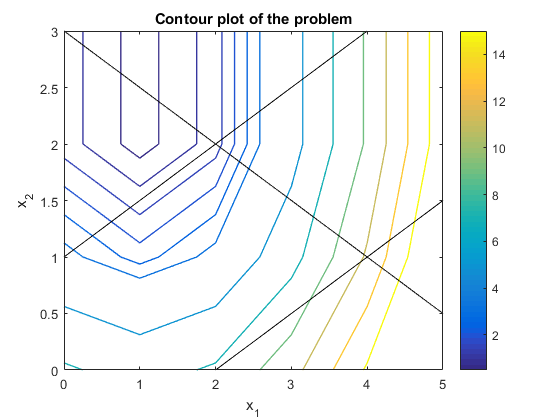
\includegraphics{exe3_contour_plot.png}
	\caption{A contour plot of the problem.}
	\label{fig:exe3_contour_plot}
\end{figure}




\subsection{Problem 4 - Markowitz Portfolio Optimization}
blablablablbal
\subsection{Problem 5 - Interior-Point Algorithm for Convex Quadratic
Programming}
blablablablbal


\end{document}
